% can be 9pt
\documentclass{sigplanconf}
\usepackage{url}
\usepackage{tikz}
\usepackage{graphicx}
\usepackage{framed}
\usepackage{color}
\usepackage{url}
\usepackage{alltt}
\usepackage{tabularx}
\usepackage{subfigure}
\usepackage{fancyhdr}
\usepackage{paralist}
\usepackage{multirow}
\usepackage{pgf}
\usepackage{nth}
\usepackage{xspace}

\usepackage{listings}
\lstset{ %
  language=Haskell,                 % the language of the code
 %%basicstyle= \scriptsize,           % the size of the fonts that are used
  %% for the code
  %%firstnumber=0, % index to start numbering at
  %%numbers=left,                      % where to put the line-numbers
  %% numberstyle=\tiny\color{gray},  % the style that is used for the
  %% line-numbers
  %% stepnumber=5,                   % the step between two line-numbers. If it's
                                  % 1, each line
  %%                              % will be numbered
  %% numbersep=5pt,                  % how far the line-numbers are from the code
  %% xleftmargin=0ex,
  %% backgroundcolor=\color{white},      % choose the background color. You must
  %% add \usepackage{color}
  %% showspaces=false,               % show spaces adding particular underscores
  %% showstringspaces=false,         % underline spaces within strings
  %% showtabs=false,                 % show tabs within strings adding
  %% particular underscores
  %% frame=single,                   % adds a frame around the code
  %% rulecolor=\color{black},        % if not set, the frame-color may be
  %% changed on line-breaks within not-black text (e.g. commens (green here))
  %% tabsize=2,                      % sets default tabsize to 2 spaces
  %% captionpos=b,                   % sets the caption-position to bottom
  %% breaklines=true,                % sets automatic line breaking
  %% breakatwhitespace=false,        % sets if automatic breaks should only
  %% happen at whitespace
  %% title=\lstname,                   % show the filename of files included
  %% with \lstinputlisting;
  %%                                 % also try caption instead of title
  %% keywordstyle=\color{blue},          % keyword style
  %% commentstyle=\color{dkgreen},       % comment style
  %% stringstyle=\color{mauve},          % string literal style
  escapeinside={@*}{*@},            % if you want to add a comment within your
                                    % code
  %% morekeywords={*,...}           % if you want to add more keywords to
  %% the set
}


%% \usepackage{tikz}
%% \usetikzlibrary{arrows,automata}

%% \usepackage{amsmath}
%% \usepackage{amsthm}

%% \newtheoremstyle{lst}
%%   {\topsep}   % ABOVESPACE
%%   {\topsep}   % BELOWSPACE
%%   {\itshape}  % BODYFONT
%%   {0pt}       % INDENT (empty value is the same as 0pt)
%%   {} % HEADFONT
%%   {}         % HEADPUNCT
%%   {5pt plus 1pt minus 1pt} % HEADSPACE
%%   {(\thmnumber{#2})}          % CUSTOM-HEAD-SPEC
%% \theoremstyle{lst}
%% \newtheorem{codenum}{lst}

\usepackage{float}
\floatstyle{boxed}
\restylefloat{figure}

%% \include{math}

\newenvironment{code}{\begin{alltt}\footnotesize}{\end{alltt}}
%% \newenvironment{cols}{\begin{tabular}{m{3.6cm}|m{3.6cm}}{Haskell} &

\newcommand{\ttp}[1]{\texttt{#1}}

\usepackage{ifthen}
\newboolean{submission}  %set to true for the submission version
\setboolean{submission}{false}
%\setboolean{submission}{true}
\ifthenelse
{\boolean{submission}}
{ \newcommand{\todo}[1]{ } } %hide todo
{ \newcommand{\todo}[1]{ {\color{blue}$<<$#1$>>$}
 }}
%\usepackage{fancyhdr}

\newcommand{\sub}[1]{\(\sb{#1}\)}

\newcommand{\undef}[1]{{\bf #1}}

%% \newcommand{\sci}[2]{\ensuremath{#1 \times 10^{#2}}}
\newcommand{\sci}[2]{\ensuremath{#1e^{#2}}}
\begin{document}

\newcommand{\xmonad}{\textsc{xmonad}\xspace}

\exclusivelicense
\conferenceinfo{Haskell~'14}{September 6, 2014, Gothenburg, Sweden.}
\CopyrightYear{2014}
\copyrightdata{978-1-4503-3041-1/14/09}
\doi{2633357.2633365}

%\titlebanner{banner above paper title}        % These are ignored unless
%\preprintfooter{}   % 'preprint' option specified.

\title{SmartCheck: Automatic and Efficient Counterexample Reduction and Generalization}
%\subtitle{UNPUBLISHED DRAFT}

\authorinfo{Lee Pike}
           {Galois, Inc.}
           {leepike@galois.com}
\maketitle

\begin{abstract}
QuickCheck is a powerful library for automatic test-case generation.  Because QuickCheck performs random testing, some of the counterexamples discovered are very large.  QuickCheck provides an interface for the user to write shrink functions to attempt to reduce the size of counterexamples.  Hand-written implementations of shrink can be complex, inefficient, and consist of significant boilerplate code.  Furthermore, shrinking is only one aspect in debugging: counterexample generalization is the process of extrapolating from individual counterexamples to a class of counterexamples, often requiring a flash of insight from the programmer.  To improve counterexample reduction and generalization, we introduce \emph{SmartCheck}.  SmartCheck is a debugging tool that reduces algebraic data using generic search heuristics to efficiently find smaller counterexamples.  In addition to shrinking, SmartCheck also automatically generalizes counterexamples to formulas representing classes of counterexamples.  SmartCheck has been implemented for Haskell and is freely available.
\end{abstract}

\category{D.2.5}{Software Engineering}{Testing and Debugging}

%% \terms
%% Languages, Verification

\keywords
property-based testing; test-case generalization; delta-debugging

\section{Introduction}\label{sec:intro}
The QuickCheck testing framework was a revolutionary step-forward in
property-based testing~\cite{qc,monadic}.  Originally designed for Haskell,
QuickCheck has been ported to other languages and is a now a widely-used testing
tool.  Because QuickCheck generates random values for testing, counterexamples
it finds may be substantially larger than a minimal counterexample.  In their
original QuickCheck paper~\cite{qc}, the authors report the following user
experience by Andy Gill:
%
\begin{quote}
Sometimes the counterexamples found are very large and it is difficult to go
back to the property and understand why it is a counterexample.
\end{quote}

That is, automated testing helps find a counterexample, but it may be a very
large counterexample.  We are left facing the \emph{shrinking problem}: consider
program $P$ modeled as a function mapping an input vector $\vec{i}$ to an output
value.  Consider property $\phi$ modeled as a function mapping the inputs of $P$
to a Boolean value that has the form $pre(\vec{i}) \Longrightarrow
post(P(\vec{i}))$, where $pre$ is a precondition on inputs and $post$ is a
postcondition on the program output.  Let $<$ be a partial order over the set of
possible inputs.  Given inputs $\vec{i}$ such that $\phi(\vec{i})$ is false, the
shrinking problem is to find inputs $\vec{j}$ such that $\phi(\vec{j})$ is false
and there exist no inputs $\vec{k}$ such that $\vec{k} < \vec{j}$ and
$\phi(\vec{k})$ is false.

In general, the problem is too expensive to solve optimally, since it requires
showing that for a set of failing inputs, there exist no strictly smaller inputs
that also cause the property to fail.  Such a demonstration requires exhaustive
testing or proof.  Solutions to the shrinking problem are therefore approximated
to efficiently discover sufficiently small inputs causing the input to fail.
Usually, the shrunk inputs are derived algorithmically (but perhaps
nondeterministically) from known larger inputs resulting in failure.

Originally, QuickCheck defines a type class
\ttp{Arbitrary} that presents a method \ttp{arbitrary} for generating random
values of a given type.  Gill added another method to the type class:
%
\begin{code}
smaller :: a -> [a]
\end{code}
%
\noindent
The purpose of \ttp{smaller} is to generate strictly smaller values, according
to some measure, from a given counterexample.  These new values are then tested
to attempt to find a smaller counterexample.  Today, \ttp{smaller} is called
\ttp{shrink}.

In industrial uses, shrinking is essential.  In describing commercial
applications of QuickCheck, Hughes has noted that ``without it [shrinking],
randomly generated failing cases would often be so large as to be almost
useless.''~\cite{qcjh}.  Hughes~\emph{et al.} also give an extended example in
which shrinking is essential in debugging telecom software~\cite{telecom}.

Defining an efficient and effective shrink method requires a good understanding
of how shrinking in QuickCheck works and the semantics of the property and
program being evaluated.  Bad definitions can be so slow or so ineffective at
shrinking that they are unusable.

\begin{figure}[ht]
\begin{code}
\scriptsize
StackSet \{current = Screen \{workspace = Workspace
\{tag = NonNegative \{getNonNegative = 0\}, layout = -1, stack =
Just (Stack \{focus = `S', up ="", down = ""\})\}, screen = 1,
screenDetail = 1\}, visible = [Screen \{workspace = Workspace
\{tag = NonNegative \{getNonNegative = 2\}, layout = -1, stack =
Nothing\}, screen = 2, screenDetail = -1\},Screen \{workspace =
Workspace \{tag = NonNegative \{getNonNegative = 3\}, layout = -1,
stack = Nothing\}, screen = 0, screenDetail = -1\}], hidden =
[Workspace \{tag = NonNegative \{getNonNegative = 1\}, layout = -1,
stack = Just (Stack \{focus = `NUL', up = "", down = ""\})\},
Workspace \{tag = NonNegative \{getNonNegative = 4\}, layout = -1,
stack = Just (Stack \{focus = `I', up = "", down = ""\})\}],
floating = fromList []\}
\end{code}
  \caption{Counterexample returned by QuickCheck for a bug-injected version of \xmonad.}
  \label{fig:xmonadex}
\end{figure}

In addition, shrinking is one side of the coin when it comes to making
counterexamples more understandable: the other side is extrapolation from
individual counterexamples to a class of counterexamples characterizing the bug.
This leap of abstraction is often implicitly made by the programmer in
determining the reason why counterexamples fail the property.  For example,
Figure~\ref{fig:xmonadex} contains a relatively small counterexample returned
when using QuickCheck to test a property in (a bug-injected version of) \xmonad,
a popular X11 window manager written in Haskell~\cite{xmonad}.  (This
counterexample uses Haskell's default \ttp{Show} instances, which uses record
syntax.)  Programmers may be familiar with having to debug a ``wall of text'' as
shown above.  What if instead a formula like the following were returned,
stating that for any well-typed values $x_0$, $x_1$, $x_2$, and $x_3$, tested, a
counterexample is found?

%% %

%% \medskip%
%% \begin{sloppypar}
%% %\footnotesize
%% \noindent%
%% \ttp{StackSet \{current = Screen \{workspace = Workspace \{tag = NonNegative
%%       \{getNonNegative = 0\}, layout = -1, stack = Just (Stack \{focus = 'S', up =
%%         "", down = ""\})\}, screen = 1, screenDetail = 1\}, visible = [Screen
%%     \{workspace = Workspace \{tag = NonNegative \{getNonNegative = 2\}, layout = -1,
%%         stack = Nothing\}, screen = 2, screenDetail = -1\},Screen \{workspace =
%%       Workspace \{tag = NonNegative \{getNonNegative = 3\}, layout = -1, stack =
%%         Nothing\}, screen = 0, screenDetail = -1\}], hidden = [Workspace \{tag =
%%       NonNegative \{getNonNegative = 1\}, layout = -1, stack = Just (Stack \{focus
%%         = `\char`\\NUL', up = "", down = ""\})\},Workspace \{tag = NonNegative
%%       \{getNonNegative = 4\}, layout = -1, stack = Just (Stack \{focus = 'I', up =
%%         "", down = ""\})\}], floating = fromList []\} }
%% \end{sloppypar}
%% \medskip%
%% \noindent

%
\begin{samepage}
\begin{code}
forall values x0 x1 x2 x3:
  StackSet
    (Screen (Workspace x0 (-1) (Just x1)) 1 1)
    x2 x3 (fromList [])
\end{code}
\end{samepage}
%
\noindent
The formula quantifies away all the irrelevant portions of the data structure
with respect to the property, so that the user can focus on the heart of the
problem in a class of counterexamples.  Given a program and large
counterexample, \emph{SmartCheck} returns such a formula.

\paragraph{SmartCheck}
Motivated by the problems of reducing and generalizing large counterexamples, we
developed SmartCheck.  SmartCheck takes a counterexample produced by some oracle
and generically minimizes and generalizes the counterexample.  After presenting
some preliminary definitions in Section~\ref{sec:preliminaries}, in
Section~\ref{sec:shrinking}, we describe SmartCheck's generic counterexample
reduction algorithm.


%% As shown in the motivating example in Section~\ref{sec:example}, SmartCheck
%% generates smaller counterexamples faster than hand-written or generated
%% QuickCheck shrinking, for some properties and programs.  (Shrinking time is
%% important in real-world uses; see Section~\ref{sec:experiments} for examples.)  



%%  than the tuple or list-truncation approaches
%% described earlier, and the size of resulting counterexamples are two-five times
%% smaller (more detailed performance numbers are given in
%% Section~\ref{sec:performance}).  Furthermore, other shrink approaches tend to
%% have ``long tails,'' meaning that for some original counterexamples, that are
%% not shrunk much or take a very long time to shrink.
%% Motivated by these limitations of QuickCheck and SmallCheck, we developed
%% \emph{SmartCheck}.

SmartCheck implements three novel approaches to automatically generalize
counterexamples, which are described in Section~\ref{sec:generalization}.  The
first algorithm universally quantifies sub-values that always fail in tests.
The second algorithm existentially quantifies sub-values for types in which
every possible variant fails the property.  For example, finding counterexamples
(\ttp{Left 2}) and (\ttp{Right True}) for the type
%
\begin{code}
\ttp{Either Int Bool}
\end{code}
%
\noindent
means there exists a counterexample regardless of the variant chosen.
Existential generalization is useful for large sum types, as found in
abstract syntax tree (AST) definitions, for example.

The third algorithm automatically strengthens properties by omitting ``similar''
counterexamples to the ones previously observed.  The algorithm is motivated by
noting that there are often multiple ways in which a property may fail; for
example, a property stating that pretty-printing an AST and then parsing it
results in the original AST may fail due to multiple bugs, such that each bug in
isolation is sufficient to cause failure.  During testing, it is useful to
discover counterexamples arising from all the bugs in one go.  In practice, the
problem is solved by discovering a counterexample \ttp{cex}, abstracting it, and
then adding a new precondition to the property that informally says ``omit
counterexamples of form \ttp{cex}.''  Adding preconditions manually is laborious
and may cause the programmer to make premature fixes to the program, if she
believes she has isolated the error before she actually does.

We describe our implementation based on generic programming in
Section~\ref{sec:implementation}; the implementation is open-source.  In
Section~\ref{sec:experiments}, we discuss some of our experiences with using
SmartCheck, including checking properties from \xmonad and a natural language
processing library.

\section{A Motivating Example}\label{sec:example}

\begin{figure}[ht]
\begin{code}
type I   = [Int16]
data T   = T I I I I I

toList :: T -> [[Int16]]
toList (T i0 i1 i2 i3 i4) = [i0, i1, i2, i3, i4]

pre :: T -> Bool
pre t = all ((< 256) . sum) (toList t)

post :: T -> Bool
post t = (sum . concat) (toList t) < 5 * 256

prop :: T -> Property
prop t = pre t ==> post t
\end{code}
  \caption{Example program and property.}
  \label{fig:initial}
\end{figure}

In this section, we motivate in more detail the challenges in shrinking
counterexamples by comparing manual approaches using QuickCheck to SmartCheck.
(We focus on shrinking rather than generalization here since counterexample
generalization is unique to SmartCheck.)  We will show how a small data type and
simple property can result in large counterexamples without any shrinking.  Then
we show the difficulty in designing an efficient shrink implementation.  We will
show a poor design before arriving at a ``canonical'' manual solution.

%% %%
%% However, even the
%% canonical solution produces significantly larger counterexamples and takes
%% significantly longer to produce them than SmartCheck, even though SmartCheck's
%% shrinking strategy is completely automatic and generic.

Consider the example in Figure~\ref{fig:initial}.\footnote{All examples and
  algorithms in this paper are presented in Haskell 2010~\cite{haskell2010} plus
  the language extensions of existential type quantification and scoped type
  variables.}  Data type \ttp{T} is a product type containing five lists of
signed 16-bit integers.  %% For our purposes, it is not important what \ttp{T}
%% models, but for concreteness, suppose it models the values in five linked lists.

Now suppose we are modeling some program that serializes values of type \ttp{T}.
The input to the program satisfies the invariant \ttp{pre}, that the sum of
values in each list of \ttp{Int16}s is less than or equal to 256.  Assuming
this, we want to show \ttp{post} holds, that the sum of all the values from
\ttp{T} is less than $5 * 256$, where five is the number of fields in \ttp{T}.
At first glance, the property seems reasonable.  But we have forgotten about
underflow; for example, since $(-20000 + -20000) \ mod \ (2^{15}) = 25536$, and
$25536 \ge 5*256$, the value
%
\begin{code}
T [-20000] [-20000] [] [] []
\end{code}
%
\noindent
satisfies \ttp{pre} but fails \ttp{post} (the \ttp{==>} operator in the figure
is implication from the QuickCheck library).

Despite the simplicity of the example, a typical counterexample returned by
QuickCheck can be large.  With standard settings and no shrinking, the average
counterexample discovered contains just over 80 \ttp{Int16} values, and over
five percent contain over 100 values.  Thus, it pays to define
\ttp{shrink}!

We might first naively try to shrink counterexamples for a data type like
\ttp{T} by taking the cross-product of shrunk values over the arguments to the
constructor \ttp{T}.  This can be expressed using Haskell's list-comprehension
notation:
%
\begin{code}
shrink (T i0 i1 i2 i3 i4) =
  [ T a b c d e | a <- shrink i0, b <- shrink i1
                , c <- shrink i2, d <- shrink i3
                , e <- shrink i4 ]
\end{code}
%
\noindent
While the above definition appears reasonable on first glance, there are two
problems with it.  First, the result of (\ttp{shrink t}) is null if any list
contained in \ttp{t} is null, in which case \ttp{t} will not be shrunk.  More
troublesome is that with QuickCheck's default \ttp{Arbitrary} instances, the
length of potential counterexamples returned by \ttp{shrink} can exceed
$10^{10}$, which is an intractable number of tests for QuickCheck to analyze.
The reason for the blowup is that shrinking a list \ttp{[a]} produces a list
\ttp{[[a]]}, a list of lists; each list is a new shrinking of the original list.
Then, we take the cross-product of the generated lists.  For the example above,
with some counterexamples, the shrinking stage may appear to execute for hours,
consuming ever more memory, without returning a result.

The first way we will try to contain the search space is by preventing the
\ttp{shrink} method from operating on numeric types.  The standard approach for
doing so is by defining a newtype wrapper:
%
\begin{code}
newtype J = J \{ getInt :: Int16 \}
\end{code}
%
\noindent
Next, a programmer might try to control the complexity by truncating lists using
%
\begin{code}
take n ls
\end{code}
%
returns the first $n$ elements \ttp{ls}.  The trade-off is quicker shrinking
with a lower probability of finding a smaller counterexample.  For example, we
might redefine shrink as follows:
%
\begin{samepage}
\begin{code}
shrink (T i0 i1 i2 i3 i4) =
  [ T a b c d e | a <- tk i0
                , b <- tk i1, c <- tk i2
                , d <- tk i3, e <- tk i4 ]
  where tk x = take 10 (shrink x)
\end{code}
\end{samepage}
%
\noindent
Call this version ``truncated shrink''.  Truncation controls the blowup of the
input-space, but the downside is that potentially smaller counterexamples may be
omitted.

Someone who understands the semantics of QuickCheck's \ttp{shrink}
implementation defines a \ttp{shrink} instance as follows:\footnote{The
  following approach was suggested to the author by John Hughes.}
%
\begin{code}
shrink (T i0 i1 i2 i3 i4) = map go xs
  where xs = shrink (i0, i1, i2, i3, i4)
        go (i0', i1', i2', i3', i4')
           = T i0' i1' i2' i3' i4'
\end{code}
%
\noindent
This ``tuple shrink'' definition does not suffer the same shortcomings: it
shrinks a value even if it contains an empty list, and the combinatorial blowup
of shrink candidates is avoided, since a pair \ttp{(a,b)} is shrunk by
attempting to shrink \ttp{a} while holding \ttp{b} constant, then attempting to
shrink \ttp{b} while holding \ttp{a} constant (and is generalized from pairs to
arbitrary tuples).  Thus, each argument to \ttp{T} is independently shrunk.

Finally, with this combination of shrinking tuples and disabling shrinking for
\ttp{Int16} values, we have an efficient and effective shrinking approach.

In early 2014, QuickCheck added the ability to derive \ttp{shrink} instances for
algebraic data types.  (The first release of the SmartCheck software was
mid-2012.)  With this new feature, the user declares
%
\begin{code}
shrink = genericShrink
\end{code}
%
\noindent
to obtain efficient shrink instances.

%% is unable to verify the property from Figure~\ref{fig:initial}, for much the
%% same reason that \ttp{shrink} is inefficient

%% For the property \ttp{prop} defined in Figure~\ref{fig:initial} (suitably
%% redefined to use SmallCheck's types).

%% to depth 16 to find the first counterexample.  Unfortunately, after a couple
%% hours of testing, Lazy SmallCheck is still checking values at depth six, and
%% the number of tests scales with respect to the depth.\footnote{All tests in
%% this paper are performed on a four-core Pentium~i7 running at 2.7GHz with 8GB
%% RAM on Fedora~16.  This test, and others unless noted, are performed using
%% interpreted Haskell under GHC 7.4.2.\todo{redo tests?}}

%% For example, for type \ttp{Int}, the depth $d$ is defined as the integers in
%% the list enumerating from $-d$ to $d$ (i.e., \ttp{[(-d)..d]}).
%% Figure~\ref{fig:smallshrink} contains functions for generating Lazy
%% SmallCheck (a variant of SmallCheck) tests by defining instances for the
%% \ttp{Serial} class.

%% Finally, even if we could overcome the problems described above with QuickCheck
%% and SmallCheck, we are left with two others.
%


%% Second, during testing, it is sometimes helpful to cover the input space
%%     by discovering different counterexamples to \ttp{prop}.  In the example in
%%     Figure~\ref{fig:initial}, one counterexample is fairly representative of
%%     others, but this is not true in general (e.g., consider properties about
%%     abstract syntax trees).  Ideally, the testing framework would automatically
%%     add a predicate characterizing a counterexample as the precondition to
%%     \ttp{prop} that strengthens the property.  That is, for a specific
%%     counterexample \ttp{ex}, we have a predicate \ttp{predEx} that holds if its
%%     argument is another counterexample that is similar to (i.e., some
%%     generalization of) \ttp{ex}.  Then we test against a new property
%% %
%% \begin{code}
%% prop' a = not (cex a) ==> prop a
%% \end{code}
%
%% \noindent
%% where \ttp{==>} is QuickCheck's implication operator that discards tests that
%% violate the precondition.
%\end{itemize}

\begin{figure}[ht]
\includegraphics[scale=0.6]{../regression/PaperExample1/out/data}
%% \includegraphics[scale=0.6]{../regression/PaperExample1/out/time-big}
%% \includegraphics[scale=0.6]{../regression/PaperExample1/out/time-small}
  \caption{Results for 1000 tests of the program in Figure~\ref{fig:initial}.}
  \label{fig:graphs}
\end{figure}

\begin{table}[ht]
\footnotesize
  \begin{center}
    \begin{tabular}{|r||c|c|c|c|c|c|}
\hline

              & \multicolumn{2}{c}{Mean} & \multicolumn{2}{c}{Std. dev.} &
\multicolumn{2}{c}{95\%}\\\hline
              & size & time  & size & time & size & time \\\hline\hline
none          & 83 & 0.013   & 22 & 0.014   & 119 & 0.023\\\hline
QC trunc      & 40 & 0.064   & 20 & 0.334   & 84 & 0.153\\\hline
QC tuple      & 10 & 0.031   & 4  & 0.039   & 16 & 0.052\\\hline
QC generic    & 13 & 0.204   & 7  & 0.946   & 28 & 0.543\\\hline
SmartCheck    & 6 & 0.021s   & 4  & 0.009   & 13 & 0.036\\\hline

    \end{tabular}
  \end{center}
  \caption{Summarizing data for the graph in Figure~\ref{fig:graphs}. Entries
    contain execution time (in seconds) and counterexample sizes (counting
    \ttp{Int16} values).}
  \label{table:results}
\end{table}

The results of our discussion above are summarized in Table~\ref{table:results}
and the corresponding graph in Figure~\ref{fig:graphs}.  First, we show the
results of no shrinking (labeled `none') as a baseline in terms of worst-case
value size.  Then we show four approaches to shrinking, as described above:
truncated shrinking (`QC trunc') with \ttp{Int16} shrinking disabled, in which
each list is truncated to 10 elements, tuple shrinking (`QC tuple'), also with
\ttp{Int16} shrinking disabled, and finally shrinking using QuickCheck's
\ttp{genericShrink} (`QC generic').\footnote{All results
  reported in the paper are with a GHC-7.6.3-compiled program, using \ttp{-O2},
  on a 2.8 GHz 4~core i7 with 16GB memory under OSX v. 10.9.2.}  We graph the
final counterexample size, measured in the total number of \ttp{Int16} values,
and execution time for counterexample discovery and shrinking.
Figure~\ref{fig:graphs} shows how many of the 1000 runs resulted in a final
value of a particular size, fitting the data with a Bezier curve.

In Table~\ref{table:results}, we summarize the graphed values and provide
execution time (including both counterexample discovery and shrinking) in
seconds as well.  For both execution time and final value size, we summarize the
mean, standard deviation, and the results at the 95th percentile.
(While we provide the standard deviations, note that the plots are not
necessarily Gaussian.)

SmartCheck produces consistently small counterexamples and does so
quickly---even smaller and faster than the best hand-tuned solution---all
without writing any problem-specific code.  Note that the `none' example
provides a lower-bound on execution time (only including counterexample
discovery time) and an upper-bound on counterexample size.  In this example, the
hand-written ``tuple shrink'' algorithm is only slightly slower and produces
slightly larger results than SmartCheck.  (QuickCheck's generic shrinking under
performs the ``tuple shrink'' likely because the generic shrink implementation
shrinks the \ttp{Int16} values.)

In Section~\ref{sec:benchmarks}, we provide additional benchmarks, but now we
turn to the design of SmartCheck.


%% More dramatic, however, are the differences in execution time.  The execution
%% times for SmartCheck include the initial counterexample generation time
%% required by QuickCheck (QC none); thus the time required by SmartCheck to
%% shrink a counterexample is on average just two hundredths of a second (0.10 -
%% 0.08).  As can be seen in the graphs, SmartCheck's execution time scales
%% linearly (like QuickCheck without shrinking).  Truncation and tuple shrinking
%% produce very long tails; the longest execution time recorded for truncation
%% shrinking and tuple shrinking are 88 seconds and 110 seconds, respectively,
%% although these outliers can vary wildly.  SmartCheck is largely insensitive
%% to the size of the original counterexample provided.

%% In regards to generalization, after shrinking the counterexample, SmartCheck
%% will also generalize it.  Note that for any \ttp{Word8} value in the first
%% argument of \ttp{T}, the counterexample still holds.  For example, SmartCheck
%% might return a counterexample of the form
%% %
%% \begin{code}
%% forall x . T x [-20000] [-20000] [] []
%% \end{code}

%% Finally, these performance results for SmartCheck are fairly generalizable to
%% other types and properties, since the algorithm is not dependent on the
%% specific program or property being checked.  However, the results are
%% particularly pronounced for counterexamples that are particularly ``deep'' or
%% ``broad'' in terms of their tree structure.  %% For programs and properties
%% for which small counterexamples are easily found, QuickCheck's shrinking is
%% perfectly acceptable.  Furthermore, user-defined shrink methods may vary
%% significantly based on the property and counterexample type, so it is not
%% always clear which implementation to compare against.





%% \begin{itemize}

%% \item an efficient counterexample reduction strategy for algebraic
%%   data types (Section~\ref{sec:shrinking});

%\item an approach to counterexample generalization, to present the user with a
%%   formula describing a set of counterexamples to a property
%%   (Section~\ref{sec:generalization});

%% \item an approach to generically strengthen a property with a precondition that
%%   characterizes an already-discovered counterexample for the purpose of finding
%%   new, dissimilar counterexamples (Section~\ref{sec:generalization});

%\item

%% \item More generally, this paper is the first to explore the idea of
%%   efficient, generic counterexample reduction and generalization for
%%   functional program testing.
% \end{itemize}


%% \noindent Moreover, the inability to quickly uncover understandable
%% counterexamples is a real-world problem with QuickCheck (or other functional
%% languages).  It works great when your tests pass,

%% \paragraph{Outline.}
%% The paper precedes as follows.  We define a type class and some definitions in
%% Section~\ref{sec:preliminaries} used in the remainder of the paper.  In
%% Section~\ref{sec:shrinking}, we describe SmartCheck's reduction algorithm for
%% efficiently shrinking large counterexamples.  In
%% Section~\ref{sec:generalization}, we turn our attention to the problem of
%% counterexample generalization.  Here, we present two algorithms for generalizing
%% counterexamples and constructing formulas for describing them.  We also discuss
%% a method for property strengthening to discover new counterexamples.  We
%% describe implementation-specific details in Section~\ref{sec:implementation},
%% and the results of some experiments in using our tool are presented in
%% Section~\ref{sec:experiments}.  Related work is given in
%% Section~\ref{sec:related}.  Finally, concluding remarks and future work are
%% presented in Section~\ref{sec:conclusions}.


%%%%%%%%%%%%%%%%%%%%%%%%%%%%%%%%%%%%%%%%%%%%%%%%
\section{Preliminaries}\label{sec:preliminaries}

SmartCheck focuses on algebraic data types represented as ``sums of products''
including recursive and mutually recursive types.  We sometimes refer to the
elements of a sum type as a \emph{variant} that is \emph{tagged} by a
constructor.  For example, the type
%
\begin{code}
Maybe a = Just a | Nothing
\end{code}
%
\noindent
contains two variants, tagged by the constructors \ttp{Just} and \ttp{Nothing},
respectively.

To present the algorithms in the following sections, we provide some definitions
in the form of methods of a \ttp{SubTypes} type class.  (SmartCheck requires
instances to be defined for data being analyzed; in
Section~\ref{sec:implementation}, we describe how instances for the type class
are derived automatically.)
%
\begin{code}
type Idx    = Int
type Size   = Int
data SubVal = forall a. SubTypes a => SubVal a

class Arbitrary a => SubTypes a where
  size    :: a -> Size
  index   :: a -> Idx -> Maybe SubVal
  replace :: a -> Idx -> SubVal -> a
  constr  :: a -> String
  constrs :: a -> [String]
  opaque  :: a -> Bool
  subVals :: a -> Tree SubVal
\end{code}
%
\noindent
The \ttp{SubTypes} type class requires QuickCheck's \ttp{Arbitrary} as a
super-class.  \ttp{SubTypes} has the following methods:
\begin{itemize}
\item \ttp{size} returns the size of a value---the number of
  constructors contained within it.
\item \ttp{index} returns a \emph{sub-value} at a breadth-first index in a
  value.
\item \ttp{replace} replaces a sub-value at a particular focus, returning the
  original value if the index is out-of-bounds.
\item \ttp{constr} returns a string representation of the constructor tagging
  the value.
\item \ttp{constrs} returns the list of all possible constructor names from the
  value's type.
\item \ttp{opaque} is false when the type of the value is an ``interesting
  type''; informally, this is a type other than a primitive type like \ttp{Int},
  \ttp{Char}, or \ttp{Bool}, and may be user-defined.  See
  Section~\ref{sec:base} for a full discussion.
\item \ttp{subVals} returns a tree of all non opaque-type sub-values.  A tree
  has the type
%
  \begin{code}
data Tree a = Node \{ rootLabel :: a
                   , subForest :: [Tree a] \}
  \end{code}
%
\end{itemize}

\noindent
To illustrate typical evaluations of the methods, consider a binary tree type:
%
\begin{code}
data T = L | B T T
\end{code}
%
\noindent
and the value \ttp{tree}, labeled with indexes in a breadth-first order:
%
\begin{code}
tree = B\sub{0} (B\sub{1} L\sub{3}
             (B\sub{4} L\sub{6} L\sub{8}))
          (B\sub{2} L\sub{5} L\sub{7})
\end{code}
%
\noindent
Here are example applications of \ttp{SubTypes} methods; in the following, we
show the indexes with respect to the value \ttp{tree}:
%
\begin{code}
size tree = 9

index tree 0  = tree
index tree 3  = (Just . SubVal) (B\sub{4} L\sub{6} L\sub{8})
index tree 12 = Nothing

replace tree 2 (SubVal L) =
  B\sub{0} (B\sub{1} L\sub{3}
        (B\sub{4} L\sub{6} L\sub{8}))
     L

constr  tree = ["B"]
constrs tree = ["B", "L"]
constrs L    = ["B", "L"]

opaque (3 :: Int) = True
opaque tree       = False
opaque L          = False

subVals (B\sub{0} (B\sub{1} L\sub{0} L\sub{1}) L\sub{2}) = SubVal
  (Node (B\sub{0} (B\sub{1} L\sub{0} L\sub{1}) L\sub{2})
        [ Node (B\sub{1} L\sub{0} L\sub{1}) [Node L\sub{0} [], Node L\sub{1} []]
        , Node L\sub{2} []
        ])
\end{code}
%
\noindent
The \ttp{SubVal} type is an existential data type, used as a generic container
for sub-values from a counterexample.  We will sometimes refer to the unwrapped
value returned by \ttp{index a i} as the \emph{$i$th sub-value of $a$}, so for
example, (\ttp{B\sub{4} L\sub{6} L\sub{8}}) is the 3rd sub-value of \ttp{tree}.
An invariant of \ttp{index} is that for any value \ttp{a}, and for the smallest
$i \geq 0$ such that
%
\begin{code}
index a i == Nothing
\end{code}
%
\noindent
then for all $0 \leq j < i$,
%
\begin{code}
index a j /= Nothing
\end{code}
\noindent
We use this invariant as a termination case in recursive algorithms over the
sub-values of a value.  (Rather than indexes into a data-structure, an
alternative representation is to use a zipper data structure~\cite{zipper} to
traverse data.  We have chosen explicit indexes to write simple tail-recursive
algorithms that can easily be transcribed to imperative languages.)

In our implementation, the \ttp{SubTypes} class and its methods depend on GHC
Generics~\cite{generics}, which we describe in Section~\ref{sec:implementation}.
For simplicity, we omit here Generics-specific super-class constraints on the
\ttp{SubTypes} class here.  Moreover, our presentation simplifies the
implementation (Section~\ref{sec:implementation}) somewhat to improve the
presentation.

%% Finally, \ttp{opaque} is true for our tree type but false for a
%% structureless type, such as \ttp{Int}.

% ------------------------------------------------------------------------------

\section{Shrinking Data}\label{sec:shrinking}
In this section, we describe how to efficiently and generically shrink algebraic
data values.  Recall the basic idea behind the \ttp{shrink} method of the
\ttp{Arbitrary} class: generate a list of values, each of which is smaller than
the current counterexample.  Each of the new values generated may not bear any
relationship to the original counterexample other than being smaller.
SmartCheck pursues an approach that searches for smaller but structurally
similar counterexamples, as we make precise below.  Perhaps the most significant
difference between SmartCheck's reduction algorithm and QuickCheck shrink
implementations is that the latter is deterministic.  SmartCheck combines
counterexample search with shrinking.

We describe the algorithm in Section~\ref{sec:reduct} and then describe
algorithmic details in Section~\ref{sec:details}.  Some optimizations to the
reduction algorithm are described in Section~\ref{sec:optimizations}.

%% Consider the problem of finding a small counterexample as a graph search
%% problem.  The set of vertexes are all possible well-typed values.  Let $<$ be
%% a partial ordering on values relating them by some size measure.  Let there
%% be an edge from vertex $v$ to $v'$ if $v < v'$ and there exists no $v''$ such
%% that $v < v'' < v'$.  The goal is to traverse the graph, starting from a
%% counterexample, to find a vertex from the set of smallest counterexamples in
%% the graph.

%% The approach taken by typical \ttp{shrink} implementations is the most naive
%% graph search algorithm: it simply generates a random set of potential vertexes
%% that are strictly smaller according to the given measure to check the property
%% against.  However, it does not exploit that the original counterexample
%% \ttp{cex} is already in a neighborhood of other likely counterexamples.  So
%% rather than choose random vertexes, it may be more efficient to test other
%% values that are closely related to \ttp{cex}.  By restricting the search to
%% \ttp{cex}'s neighborhood, a smaller counterexample might be missed, and only a
%% local minimum is returned.  However, with a large set of values, finding a
%% global minimum by random sampling vertexes in the graph is possible but too
%% inefficient.

\subsection{Reduction Algorithm Overview}\label{sec:reduct}
The algorithm we present for efficiently searching for new counterexamples is an
instance of greedy breadth-first search over a tree structure that represents a
value.  At each node, during the traversal, we generate arbitrary
structurally smaller sub-values and build a new value from that, leaving
the remainder of the tree unchanged.  By a \emph{structurally
  smaller value}, we mean one with fewer constructors.  We continue until we
reach a fixed-point.


\begin{figure}[ht]
  \lstset{caption={}
%         ,xleftmargin=5ex,firstnumber=0,numbers=left
         }
  \begin{code}
getSize :: SubVal -> Size
getSize (SubVal a) = size a

newVals :: Size -> Int -> SubVal -> IO [SubVal]
newVals sz tries (SubVal a) =
  replicateM tries s where
  s = liftM SubVal (\undef{sizedArbitrary} sz a)

reduce :: SubTypes a
  => ScArgs -> (a -> Property) -> a -> IO a
reduce args prop cex = reduce' 1
  where
  reduce' idx
    | Just v <- index cex idx
    = do vs <- newVals (getSize v)
                 (scMaxReduce args) v
         case test cex idx vs prop of
           Nothing -> reduce' (idx+1)
           Just a  -> reduce args prop a
    | otherwise = return cex

test :: SubTypes a => a -> Idx -> [SubVal]
     -> (a -> Property) -> Maybe a
test cex idx vs prop = go vs
  where
  go []      = Nothing
  go (v:vs') =
    let cex' = replace cex idx v in
    if \undef{pass} prop cex' then go vs'
      else Just cex'
  \end{code}
  \caption{Counterexample reduction algorithm.\label{fig:reduction}}
\end{figure}

Figure~\ref{fig:reduction} shows the reduction algorithm.  In this algorithm and
subsequent algorithms in the paper, functions in {\bf bold font} are left
undefined but their implementation is described in the text.  The function
\ttp{reduce} takes flags to customize the algorithm's behavior, a counterexample
\ttp{cex}, and the property \ttp{prop}.  The reduction begins at the first
proper sub-value of \ttp{cex}; call it \ttp{v} (this is an optimization
described in Section~\ref{sec:variant}).  When the index \ttp{idx} becomes
out-of-bounds and returns \ttp{Nothing}, the algorithm terminates.  Otherwise, a
list of new random values are generated.
%
\begin{code}
sizedArbitrary :: SubTypes a => Size -> a -> IO a
\end{code}
%
\noindent
generates a new value \ttp{v'} having the same type as \ttp{v} and that is
strictly smaller (with respect to the \ttp{size} method) than \ttp{v}.  Just
like QuickCheck's \ttp{arbitrary} method, \ttp{sizedArbitrary} generates
successively larger counterexamples when generating new values with which to
replace a sub-value.

The flag \ttp{scMaxReduce} is the maximum number of tries to discover a new
counterexample by replacing \ttp{v} in \ttp{cex} and testing it.  The result of
\ttp{pass prop cex'} for
%
\begin{code}
pass :: (a -> Property) -> a -> Bool
\end{code}
%
\noindent
holds if \ttp{cex'} satisfies the property \ttp{prop}.  The property may be a
conditional, in which case the value must pass the precondition as well as the
consequent for \ttp{pass} to return \ttp{True}.  If no failure is found, we move
to the next sub-value of \ttp{cex} and continue.  However, if a new smaller
counterexample \ttp{cex'} is found, we start a new breadth-first traversal of
\ttp{cex'}, attempting to shrink it further.

The algorithm is guaranteed to terminate: informally, the measure for the
function is that either the index increases or the size of the counterexample
being evaluated decreases.  The algorithm's complexity is
$\mathcal{O}(n^2)$, where $n$ is the number of constructors in the
counterexample, assuming that generating new sub-values and testing them is done
in constant time.

\subsection{Reduction Algorithm Details}\label{sec:details}
Having described the reduction algorithm, there are two important details about
its design we describe below.

\subsubsection{Variant Counterexample Hypothesis}\label{sec:variant}
A motivation for the design of the reduction algorithm is something we call the
\emph{variant counterexample hypothesis}: in the search space of possible values
from a given type \ttp{T}, if a known counterexample \ttp{cex} is a variant
\ttp{v} of \ttp{T}, then it is most probable that other counterexamples are also
from variant \ttp{v}.  As an example supporting the hypothesis, consider a
property about unintended variable capture over a language's parse tree
represented by a sum type with constructors for module imports, function
definitions, and global-variable assignments, respectively.  A function
definition counterexample can only be reduced to smaller function definition
counterexamples, the only construct in which variable capture is possible.

Recall that the algorithm begins at the \emph{first} sub-value of the
counterexample rather than the zeroth sub-value so that the variant of the
counterexample remains the same.  No invariant of the algorithm would be
violated by beginning with the zeroth sub-value, and in particular, the
algorithm would still terminate.

Incidentally, QuickCheck's generic shrink implementation is fundamentally build
around the variant counterexample hypothesis.  For a given counterexample
\ttp{cex}, smaller candidates produced by \ttp{shrink} contain only the
constructors found in \ttp{cex} as opposed to just the outermost constructor, as
in SmartCheck.  Sometimes shrinking gets ``stuck'' at a local minimum due to a
lack of entropy in generating smaller candidates.

The hypothesis may be unsuitable for some properties, in which case SmartCheck
(and especially QuickCheck) may potentially fail to discover a smaller
counterexample.  However, in Sections~\ref{sec:existential}
and~\ref{sec:precondition}, we describe approaches to generalize counterexamples
based on discovering new counterexample variants.  These generalization
techniques are executed in an (optional) generalization phase, run after the
reduction phase, in which this hypothesis is implemented.


%% Another way to motivate the hypothesis is that searching the space of
%% possible counterexamples by generating \emph{any} well-typed value that is
%% strictly smaller than the original counterexample is something we have seen
%% before: it is precisely the naive approach to implementing \ttp{shrink}!

%% \subsubsection{Conditional Properties}
%% A QuickCheck property may be a conditional of the form
%% %
%% \begin{code}
%% prop a = pre a ==> prop' a
%% \end{code}
%% %
%% \noindent
%% such that \ttp{prop} is true if the precondition (\ttp{pre a}) is false or
%% (\ttp{prop' a}) holds.  In practice, conditionals are used to restrict the set
%% of values tested; values that fail the precondition are discarded.  Thus, the
%% call to \ttp{pass} in the reduction algorithm only considers a potential
%% counterexample \ttp{cex} to have failed if it passes the property's precondition
%% and fails the consequent.

\subsubsection{Opaque Types}\label{sec:base}

SmartCheck focuses on efficiently shrinking and generalizing large data
structures.  It is not intended as a general replacement for QuickCheck's
\ttp{shrink} method.  Consequently, SmartCheck ignores ``primitive'' types
without value constructors, such as \ttp{Char}, \ttp{Int}, and \ttp{Word16}.
Our experience is that for the kinds of properties with counterexamples that
contain massive data structures, shrinking primitive types does not
significantly help in understanding them.  Furthermore, by ignoring these types
by fiat, shrinking time is dependent only on the size of a data structure as
measured by the number of constructors.

We generalize the idea of ignoring primitive types by introducing the concept of
\emph{opaque types}.  If the reduction algorithm encounters an opaque type, it is
ignored.  Opaque types include the primitive types mentioned above, but the
user can declare any substructure in a data type to be an opaque type by
providing custom instances.  Doing so effectively treats values from that type
as ``black boxes'', making SmartCheck more efficient if the user knows that some
portion of the structure cannot be shrunk or is irrelevant to the property.

Opaque types can be conditional.  For example, the user may want lists to be
shrunk in general, unless the elements of the list are opaque themselves.  Such
a definition is possible.  Sometimes shrinking primitive types is imperative;
for example, to determine if there is a relationship between two integers in a
counterexample.

Opaque types are defined by providing the method for \ttp{opaque} in the
\ttp{SubTypes} type class.


%% The number of constructors in an algebraic data value primarily determines how
%% large it is.  In some cases, the size of fields that come from primitive
%% types, like \ttp{Int} or \ttp{Char}, have less of a role in understanding a
%% counterexample, so in general, we want to prevent our reduction algorithm from
%% spending time shrinking values from these types.


%% By default, this includes ``primitive'' types (e.g., \ttp{Int}, \ttp{Word},
%% \ttp{Float}, \ttp{Bool}, and \ttp{Char}).  We also treat recursive container
%% types like lists specially: lists of opaque types are considered to be opaque
%% types themselves.  This prevents the algorithm from analyzing, for example,
%% strings.  A list of non-opaque-types, however, is shrunk by the algorithm.

%% Conversely, if the user wishes to shrink types that are treated as opaque by
%% default, she can sometimes do so before handing the counterexample to
%% SmartCheck, say by using QuickCheck's shrink instances to shrink base types
%% while leaving the remaining structure for SmartCheck to shrink.  In the future,
%% depending on user experiences, default instances for types can be removed so
%% that SmartCheck's reduction algorithm does not ignore values from those types.

\subsection{Reduction Algorithm Optimizations}\label{sec:optimizations}
The reduction algorithm description above omits some details and optimizations
we describe here.

\subsubsection{Sub-value Counterexample Hypothesis}\label{sec:subval}
Sometimes, a counterexample fails a property due to a sub-value nested deep
inside the counterexample.  The rest of the value is irrelevant.  We call this
the \emph{sub-value counterexample hypothesis.}  Thus, one way to efficiently
search the space of potential counterexamples is to test a counterexample's
(well-typed) sub-values.

For example, consider a simple calculator language containing constants,
addition, and division, together with an evaluator that checks if the divisor is
0 and returning \ttp{Nothing} in that case:
%
\begin{code}
data Exp = C Int
         | Add Exp Exp
         | Div Exp Exp
\end{code}
%
\begin{code}
eval :: Exp -> Maybe Int
eval (C i) = Just i
eval (Add e0 e1) =
  liftM2 (+) (eval e0) (eval e1)
eval (Div e0 e1) =
  let e = eval e1 in
  if e == Just 0 then Nothing
    else liftM2 div (eval e0) e
\end{code}
%
\noindent
Now consider the property \ttp{prop\_div}, claiming that if \ttp{divSubTerms}
holds on an expression, then the evaluator returns \ttp{Just} a value:
%
\begin{code}
divSubTerms :: Exp -> Bool
divSubTerms (C _)         = True
divSubTerms (Div _ (C 0)) = False
divSubTerms (Add e0 e1)   =  divSubTerms e0
                          && divSubTerms e1
divSubTerms (Div e0 e1)   =  divSubTerms e0
                          && divSubTerms e1

prop_div e = divSubTerms e ==> eval e /= Nothing
\end{code}
%
Testing \ttp{prop\_div}, we might have a counterexample like the following:
%
\medskip%
\begin{sloppypar}
\small
\noindent%
\ttp{Add (Div (C 5) (C (-12))) (Add (Add (C 2) (C 4)) (Add (C 7) (Div (Add (C 7)
  (C 3)) (Add (C (-5)) (C 5)))))}
\end{sloppypar}
\medskip%
%
\noindent
The cause is that \ttp{divSubTerms} fails to check whether the
divisor evaluates to zero.  In the counterexample, the culprit is a buried
sub-value:
%
\begin{code}
Div (Add (C 7) (C 3)) (Add (C (-5)) (C 5))
\end{code}
%
\noindent
Thus, when attempting to shrink an \ttp{Exp} value, it pays to test whether a
sub-value itself fails the property.

%% and consider an interpreter for the language that returns \ttp{Nothing} if
%% division-by-zero is encountered and (\ttp{Just x}), where \ttp{x} is the result
%% of the computation, otherwise:
%% %
%% \begin{code}
%% eval :: Exp -> Maybe Int
%% eval (C i) = Just i
%% eval (Add e0 e1) =
%%   liftM2 (+) (eval e0) (eval e1)
%% eval (Div e0 e1) =
%%   let e = eval e1 in
%%   if e == Just 0 then Nothing
%%     else liftM2 div (eval e0) e
%% \end{code}
%% %
%% \noindent
%% Suppose we restrict the set of programs with the following predicate:
%% %
%% \begin{code}
%% divSubTerms :: Exp -> Bool
%% divSubTerms (C _)         = True
%% divSubTerms (Div _ (C 0)) = False
%% divSubTerms (Add e0 e1)   =    divSubTerms e0
%%                             && divSubTerms e1
%% divSubTerms (Div e0 e1)   =    divSubTerms e0
%%                             && divSubTerms e1
%% \end{code}
%% %
%% and then test the property
%% %
%% \begin{code}
%% prop_div e = divSubTerms e ==> eval e /= Nothing
%% \end{code}
%% %
%% \noindent
%% The property \ttp{prop\_div} turns out to be false; for example,
%% %
%% \begin{code}
%% Div (C 1) (Div (C 0) (C 1))
%% \end{code}
%% %
%% \noindent
%% is a counterexample.  In the predicate case
%% %
%% \begin{code}
%% divSubTerms (Div _ (C 0)) = False
%% \end{code}
%% %
%% \noindent
%% we forgot to recur on the divisor.

%% %% \begin{figure}[ht!]
%% %%   \caption{Typical counterexample from QuickCheck with no user-defined
%% %%     \ttp{shrink} function.}
%% %%   \label{fig:div-cex}
%% %% \end{figure}

%% A typical counterexample returned by QuickCheck, with a \ttp{shrink} function
%% implemented, is as follows:%
%% %
%% \medskip


%% \begin{sloppypar}
%% %\makebox[\textwidth]{
%% \noindent%
%% \ttp{Div (Add (Div (Div (C (-12)) (C 22)) (Add (C 10) (C (-5)))) (Div (Add (C
%%   30) (C 12)) (C (-18)))) (Div (Div (C (-20)) (C 32)) (Div (C 10) (C (-8))))}
%% \end{sloppypar}
%% \medskip%

%% \noindent
%% It turns out that the culprit is the sub-value
%% %
%% \begin{code}
%% Div (Div (C (-20)) (C 32)) (Div (C 10) (C (-8)))
%% \end{code}
%% %
%% \noindent
%% Thus, while analyzing the counterexample above

\begin{figure}
\begin{code}
reduceOpt :: forall a . SubTypes a
  => ScArgs -> (a -> Property) -> a -> IO a
reduceOpt args prop cex = reduce' 1
  where
  reduce' idx
    | Just v <- index cex idx
    = case testHole v of
        Nothing -> test' v idx
        Just a  -> reduceOpt args prop a
    | otherwise = return cex

  test' v idx = do
    vs <- newVals (getSize v) (scMaxReduce args) v
    case test cex idx vs prop of
      Nothing -> reduce' (idx+1)
      Just a  -> reduceOpt args prop a

  testHole (SubVal a) = do
    a' <- \undef{cast} a :: Maybe a
    if \undef{pass} prop a' then Nothing else Just a'
\end{code}
  \caption{Reduction algorithm with the sub-value counterexample optimization.}
  \label{fig:reduce0}
\end{figure}

Generalizing the scenario, during the reduction algorithm's breadth-first
search through a counterexample \ttp{cex}'s sub-values, we may happen upon a
sub-value \ttp{cex'} that has the same type as \ttp{cex} and fails the property
(while passing any preconditions).  In this case, we can return \ttp{cex'}
directly, and rerun the reduction algorithm on \ttp{cex'}.  In
Figure~\ref{fig:reduce0}, we show an updated reduction algorithm, \ttp{reduceOpt},
that implements this optimization.  The function \ttp{testHole} tests the
current sub-value and if it fails the property, then we run the execution
algorithm on the sub-value directly.


\subsubsection{Bounding Counterexample Exploration}

SmartCheck's implementation contains flags to allow the user to customize its
behavior.  Three flags that are relevant to the reduction algorithm are the
following:
%
\begin{code}
scMaxReduce :: Int
scMaxSize   :: Int
scMaxDepth  :: Maybe Int
\end{code}
%
\noindent
The \ttp{scMaxReduce} flag controls the number of values generated by the
reduction algorithm for each sub-value analyzed.  \ttp{scMaxSize} controls the
maximum size of values generated to replace sub-values by the reduction
algorithm.  Thus, new sub-values must be strictly smaller than the minimum of
\ttp{scMaxSize} and the size of the sub-value being replaced.  Finally,
\ttp{scMaxDepth} determines the maximum depth in the counterexample the
reduction algorithm should analyze.  A value of \ttp{Nothing} means that the
counterexample should be exhaustively reduced, as the algorithm is presented in
Figure~\ref{fig:reduction}.  For example, the depth of a list is determined by
its length, and the depth of the binary tree defined in Section~\ref{sec:reduct}
is determined by the function \ttp{depth}:
%
\begin{code}
depth L         = 0
depth (B t0 t1) = 1 + max (depth t0) (depth t1)
\end{code}
%
\noindent
Of the flags, \ttp{scMaxDepth} is the most important for controlling
efficiency, particularly for large product types with significant ``fan out''.
The number of sub-values of a product type value can grow exponentially with
respect to the depth.  Furthermore, note that as the reduction algorithm
descends further, there is less chance to reduce the size of the value overall,
since smaller and smaller sub-values are replaced.


\section{Counterexample Generalization}\label{sec:generalization}

Small counterexamples make debugging easier, but they are just half the battle.
To go from a specific counterexample to the required fix in a program, the
programmer must have a flash of insight in which she generalizes the
counterexample to a set of counterexamples for which the program and property
fails.  The generalization step is an important yet under-appreciated step in
the debugging process.  A characterizing formula reduces the noise in favor of
the signal by abstracting away portions of a large counterexample that are
irrelevant to why it violates the property.

The characterization of counterexamples that most helps the programmer should
strike a middle ground.  A single counterexample is too specific.  On the other
hand, the property itself is a formula that over-approximates the failing
inputs.  In this section, we describe two kinds of formula that fall between
these two extremes that we call universal and existential sub-value
generalization, respectively.  We then describe a third approach to
generalization to automatically strengthen a property's precondition to obtain
new counterexamples.

In SmartCheck, the universal and existential generalization phases run after a
counterexample has been minimized.  Precondition strengthening is used when
iteratively generating multiple counterexamples, so it is interspersed with
counterexample reduction.

\subsection{Universal Sub-Value Generalization}\label{sec:universal}
Consider again the calculator language from Section~\ref{sec:subval}.  The
property \ttp{prop\_div} is violated for any numerator, so we might generalize a
counterexample like
%
\begin{code}
Div (Add (C 7) (C 3)) (Add (C (-5)) (C 5))
\end{code}
%
\noindent
by the formula
%
\begin{code}
forall x . Div x (Add (C (-5)) (C 5))
\end{code}
%
\noindent
since any dividend results in divide-by-zero for the given divisor.  Not only do
the generalizations assist the programmer's insight, but they reduce the sheer
size of the counterexample.  We call the kind of formula just shown
\emph{universal sub-value generalization} and it is implemented in SmartCheck.

An extrapolation algorithm performs universal sub-value generalization.  The
basic idea is as follows: for a counterexample \ttp{cex} and a property
\ttp{prop}, a breadth-first search over the sub-values of the \ttp{cex} is
performed.  For each sub-value, the algorithm generates new sub-values and
replaces them in \ttp{cex} to create a list of new potential counterexamples.
If no new value satisfies the property, then we extrapolate, claiming that for
\emph{any} new value replacing that sub-value in \ttp{cex}, the property will
fail.

\begin{figure}
  \begin{code}
subTrees :: SubTypes a => a -> Idx -> [Idx] -> Bool
subTrees cex idx = any (\undef{subTree} cex idx)

extrapolate :: SubTypes a
  => ScArgs -> a -> (a -> Property) -> IO [Idx]
extrapolate args cex prop = extrapolate' 1 []
  where
  extrapolate' idx idxs
    | subTrees cex idx idxs
    = extrapolate' (idx+1) idxs
    | Just v <- index cex idx = mkNewVals v
    | otherwise = return idxs
    where
    mkNewVals v = do
      vs <- newVals (scMaxSize args)
                    (scMaxForall args) v
      extrapolate' (idx+1)
        (if allFail args cex idx vs prop
           then idx:idxs else idxs)

allFail :: SubTypes a => ScArgs -> a -> Idx
  -> [SubVal] -> (a -> Property) -> Bool
allFail args cex idx vs prop =
  length res >= scMinForall args && and res
  where
  res  = mapMaybe go vs
  go   = \undef{fail} prop . replace cex idx
  \end{code}
  \caption{Universal sub-value generation algorithm.}
  \label{fig:universal}
\end{figure}

The extrapolation algorithm is shown in Figure~\ref{fig:universal}; let us sketch
its specification.  The algorithm is similar to the reduction algorithm in
Figure~\ref{fig:reduction} (and in the implementation, the algorithms are
generalized and combined).  The function \ttp{extrapolate} returns a list of
indexes to be generalized in the original counterexample.  In the recursive
function \ttp{extrapolate'}, there is a function guard with a call
%
\begin{code}
subTree cex idx0 idx1
\end{code}
%
\noindent
where \ttp{subTree} has the type
%
\begin{code}
subTree :: SubTypes a => a -> Idx -> Idx -> Bool
\end{code}
%
\noindent
The value
%
\begin{code}
subTree cex idx0 idx1
\end{code}
%
is true if in \ttp{cex}, the value at index \ttp{idx0} is a child of index
\ttp{idx1} in a tree representation of \ttp{cex} (i.e., \ttp{subVals cex}).  The
\ttp{subTrees} guard prevents the algorithm from trying to generalize sub-values
that are abstracted away already since their parents have been generalized.
New sub-values are generated by \ttp{newVals}, shown in
Figure~\ref{fig:reduction}.

The function \ttp{allFail} takes a counterexample \ttp{cex}, an index into
\ttp{cex}, a list of new sub-values, and a property.  It returns true if no new
values satisfy the property.  The function
%
\begin{code}
fail :: (a -> Property) -> a -> Maybe Bool
\end{code}
%
\noindent
is roughly the dual of \ttp{pass} in the reduction algorithm: (\ttp{fail
  prop cex}) returns (\ttp{Just True}) if \ttp{cex} passes \ttp{prop}'s
precondition but fails the property, (\ttp{Just False}) if \ttp{cex}
non-trivially satisfies \ttp{prop}, and \ttp{Nothing} if \ttp{cex} fails
\ttp{prop}'s precondition.

Like in the reduction algorithm, user-specified flags bound the behavior of the
algorithm.  We bound the size of values to generate by the flag \ttp{scMaxSize},
which is independent of the size of the particular sub-value.  The flag
\ttp{scMaxForall} is the analogue of the \ttp{scMaxReduce} flag, determining the
number of values generated in trying to generalize a value.  The flag
\ttp{scMinForall} is the minimum number of \ttp{Just False} results required
from \ttp{fail} to extrapolate from failed tests to a universal claim.  So, for
example, if \ttp{scMaxForall} is set to 30 and \ttp{scMinForall} is set to 20,
we generate 30 new values, 20 of which must pass the precondition but fail the
property to claim the counterexample can be generalized.

The algorithm's complexity is $\mathcal{O}(n)$, where $n$ is the number of
constructors in the counterexample.  Again, we assume that the cost for
generating random values and testing them at each index is constant.

\paragraph{Soundness}
The extrapolation algorithm is unsound in two ways.  First, it extrapolates from
a set of counterexamples to a universal claim, similar to QuickSpec or
Daikon~\cite{qs,daikon}.  By tuning the parameters, the risk of an unsound
generalization is reduced by requiring more or larger values to fail the
property.

Second, in some cases, a formula may be returned that is overly general.  For
example, consider the counterexample in which both arguments of the outermost
\ttp{Add} constructor contain values causing the failure:
%
\begin{code}
Add (Div (C 1) (Add (C (-2)) (C 2)))
    (Div (C 0) (Add (C (-1)) (C 1)))
\end{code}
%
\noindent
Since no matter what random value the first field of the outermost \ttp{Add}
constructor is replaced with, the property fails by \ttp{Add}'s second field,
and vice versa for replacing the second field.  Consequently, the universal
generalization algorithm might return the formula
\noindent
%
\begin{code}
forall values x0 x1 . Add x0 x1
\end{code}
%
\noindent
%% An over-generalized formula is only a problem when generalizing without
%% minimizing the counterexample first, as pointed out to the author by John
%% Hughes, so in practice with SmartCheck, this form of unsoundness does not arise.
%% However, if one were to generalize without shrinking first, 
The reader should read a universally quantified formula as shorthand for
quantifying each variable independently and taking the conjunction of formulas.
For example, instead of
%
\begin{code}
forall values x0 x1 . Add x0 x1
\end{code}
%
\noindent
one should read
%
%
\begin{code}
      forall values x0 .
        Add x0 (Div (C 0) (C (-1)) (C 1))
  and forall values x1 .
        Add (Div (C 1) (C (-2)) (C 2)) x1
\end{code}


\subsection{Existential Sub-Value Generalization}\label{sec:existential}

Sum types denote choice in a data type.  Sometimes, a property over a sum type
fails because there is a bug for some of the variants but not others.  For
example, recall again the calculator language from Section~\ref{sec:subval}.  The
no-division-by-zero property fails only for values that contain a variant tagged
with the \ttp{Div} constructor.  Recall again the generalized counterexample
from Section~\ref{sec:generalization}:
%
\begin{code}
forall x . Div x (Add (C (-5)) (C 5))
\end{code}
%
\noindent
Because the divisor does not generalize, we know there is something special
about it that causes failure.  But we might wonder if there is something special
about variants tagged by the \ttp{Add} constructor, or might we finding failing
sub-values with the other variants.

We therefore introduce another kind of generalization we call \emph{existential
  sub-value generalization}.  In this generalization, if there is a
counterexample containing every possible variant as a sub-value, then we
abstract it.  For example, suppose that \ttp{divSubTerms} had no equation
%
\begin{code}
divSubTerms (Div _ (C 0)) = False
\end{code}
%
\noindent
Then the following would all be counterexamples:
%
\begin{code}
Div (Add (C 3) (C 2)) (C 0)
Div (C 7) (Add (C (-5)) (C 5))
Div (C (-2)) (Div (C 0) (C 1))
\end{code}
%
\noindent
Because there are only three variants in the type, we have found counterexamples
built from each of them in the divisor.  We therefore can claim the following
formula holds:
%
\begin{code}
forall values x .
  forall constructors c .
    there exist arguments \(\stackrel{\rightarrow}{y}\) .
      such that Div x (c\(\stackrel{\rightarrow}{y}\))
\end{code}
%
\noindent
We therefore present an existential sub-value generalization algorithm that
performs constructor generalization.  Like with the other algorithms, this
algorithm also performs a breadth-first search over a counterexample.

\begin{figure}
  \begin{code}
subConstr :: SubVal -> String
subConstr (SubVal a) = constr a

subConstrs :: SubVal -> [String]
subConstrs (SubVal a) = constrs a

sumTest :: SubTypes a => ScArgs -> a
  -> (a -> Property) -> [Idx] -> IO [Idx]
sumTest args cex prop exIdxs = sumTest' 1 []
  where
  sumTest' idx idxs
    | subTrees cex idx (exIdxs ++ idxs)
    = sumTest' (idx+1) idxs
    | Just v <- index cex idx = fromSumTest v
    | otherwise = return idxs
    where
    fromSumTest v = do
      vs <- newVals (scMaxSize args)
              (scMaxExists args) v
      sumTest' (idx+1)
        (if constrFail cex idx vs prop
           (subConstr v) (subConstrs v)
           then idx:idxs else idxs)

constrFail :: SubTypes a => a -> Idx -> [SubVal]
  -> (a -> Property) -> String -> [String] -> Bool
constrFail cex idx vs prop con allCons =
  constrFail' [con] vs
  where
  constrFail' cons vs'
    | length cons == length allCons = True
    | null vs'                      = False
    | go v == Just True
    = constrFail' (c:cons) (tail vs')
    | otherwise
    = constrFail' cons (tail vs')
    where
    v  = head vs'
    c  = subConstr v
    go = fail prop' . replace cex idx
    prop' a = c `notElem` cons ==> prop a
  \end{code}
  \caption{Existential sub-value generation algorithm.}
  \label{fig:constrs}
\end{figure}

We show the algorithm in Figure~\ref{fig:constrs}.  The function \ttp{sumTest}
takes a set of flags, a counterexample, a property, and a list of indexes that
have already been generalized---perhaps by the extrapolation algorithm in
Figure~\ref{fig:universal}.  The list of course may be empty if no sub-values
have been previously extrapolated.  In a call to \ttp{subTrees}, discussed in
Section~\ref{sec:universal}, the guard prevents constructor generalization if
the current index is a sub-value of a previously generalized value.  Otherwise,
a list of well-typed new values are generated by a call to \ttp{newVals}, as
shown in Figure~\ref{fig:reduction}.  In the arguments to \ttp{newVals}, we
bound the size of values generated with \ttp{scMaxSize} as before, and bound the
number of values generated with the flag \ttp{scMaxExists}.  Because values are
randomly generated, for ``wide'' sum-types (i.e., with a large number of
constructors), \ttp{scMaxExists} should be large enough to ensure with high
probability that each variant is generated.

The function \ttp{constrFail} returns true if we replace the sub-value at index
\ttp{idx} in counterexample \ttp{cex} with every possible variant given the type
and construct a counterexample to the property.  There are four guards to the
recursive function \ttp{constrFail'}: the first guard holds if the list of
constructors tagging variants in which a counterexample is found is equal in
size to the list of all possible constructors for the type.  The second guard
tests whether the set of test values is null; if so (and if the first guard
fails), then we have exhausted test values before finding all possible failing
variants.  Third, for a specific sub-value \ttp{v}, we test whether it fails the
property.  If so, we add its constructor to the list of constructors.
Otherwise, we simply recurse.  Note in the definition of \ttp{prop'}, we add an
additional precondition that the current constructor is not an element of
constructors already seen.  Thus, (\ttp{go v}) returns
%
\begin{code}
\ttp{Just True}
\end{code}
%
\noindent
if
%
\begin{code}
\ttp{replace cex idx v}
\end{code}
%
passes this precondition (and any other preconditions of \ttp{prop}), but fails
the property.

Unlike universal sub-value generalization, existential sub-value generalization
is sound.  The existential claim is only that for each variant, there exists at
least one counterexample.

This algorithm's complexity is also $\mathcal{O}(n)$, where $n$ is the number of
constructors in the counterexample.

\subsection{Automated Precondition Strengthening}\label{sec:precondition}
The universal and existential generalization algorithms generalize a
counterexample, but in the ``neighborhood'' of the original counterexample.  In
particular, all generalizations are from the same variant as the original
counterexample.  To help the programmer in the generalization step, we would
also like a way to test the property again, ensuring we get counterexamples (if
they exist) outside of the neighborhood of the original one.

\begin{figure}[ht!]
  \begin{center}
    \includegraphics[scale=0.49]{Figs/cex-gen}
   \end{center}
  \caption{Counterexample generalization.}
  \label{fig:cex-gen}
\end{figure}

Figure~\ref{fig:cex-gen} illustrates a property of the form (\ttp{pre ==>
  post}).  Points are specific counterexamples that satisfy the precondition but
fail the post-condition, and the enclosing oval represents the generalization of
counterexamples resulting from either universal or existential generalization.
Our goal is to find additional counterexamples in the shaded region.  As new
counterexamples are discovered in the shaded region (and generalized), the
counterexample space becomes covered until no more classes of counterexamples
exist or it becomes too difficult for the testing framework to discover them.

\begin{figure}
  \begin{code}
matchesShapes :: SubTypes a
  => a -> [(a,[Idx])] -> Bool
matchesShapes d = any (matchesShape d)

matchesShape :: SubTypes a
  => a -> (a, [Idx]) -> Bool
matchesShape a (b, idxs)
  | constr a /= constr b = False
  | Just a' <- aRepl
  = let x = subForest (subVals a') in
    let y = subForest (subVals b)  in
    all foldEqConstrs (zip x y)
  | otherwise = False
  where
  updateA idx d =
    fmap (replace d idx) (index b idx)
  aRepl = foldl go (Just a) idxs where
    go ma idx | Just x <- ma = updateA idx x
              | otherwise    = Nothing
  foldEqConstrs ( Node (SubVal l0) sts0
                , Node (SubVal l1) sts1 )
    | constr l0 == constr l1 =
      all foldEqConstrs (zip sts0 sts1)
    | otherwise              = False
  \end{code}
  \caption{Shape matching algorithm.}
  \label{fig:matches}
\end{figure}

Figure~\ref{fig:matches} shows the shape-matching algorithm used for precondition
strengthening.  The function takes a candidate counterexample and a list of
previous counterexamples, together with the indexes at which they have been
generalized.  The basic idea of the algorithm is to determine whether two values
have the same ``shape''.  We consider two values to have the same
shape if in their respective tree representations, their constructors at each
node in the tree match, ignoring all opaque types (Section~\ref{sec:base}).
That is, for values \ttp{a} and \ttp{b},
%
\begin{code}
subVals a == subVals b
\end{code}
%
\noindent
Furthermore, indexes that have been universally generalized (and all their
children) match any value, since a universally generalized index indicates that
counterexamples have been found for any possible constructor.  In our
implementation, we also consider existentially generalized indexes to match any
value.  Doing so is a design choice that is more aggressive about covering the
space of counterexamples at the risk of omitting some.

To understand the shape matching algorithm, consider a few values of type
\ttp{Exp}, defined in Section~\ref{sec:subval}:
%
\begin{code}
e0 = Div (C 1) (C 2)
e1 = Div (C 1) (C 3)
e2 = Div (Add (C 1) (C 2)) (C 7)
e3 = Div (Div (C 8) (C 2)) (C 7)
\end{code}
%
\noindent
Then the following hold:
%
\begin{code}
matchesShape e0 (e1, [])  == True
matchesShape e1 (e2, [])  == False
matchesShape e1 (e2, [1]) == True
matchesShape e3 (e2, [1]) == True
\end{code}
%
The first equation holds because we ignore opaque types, so the arguments to
\ttp{C} are considered equal.  The second equation fails because at index 1,
\ttp{e1} contains the constructor \ttp{C} and \ttp{e2} contains the constructor
\ttp{Add}.  If, however, index 1 has been generalized, then we ignore the sub-value
at index 1, and they match (the third equation).  The same reasoning holds for
the fourth equation.

SmartCheck can run in a real-eval-print loop (REPL), discovering new
counterexamples, shrinking them, generalizing them, and then repeating.  In each
iteration of the REPL, the property precondition is strengthened, requiring that
\ttp{matchesShape} does not hold on the current counterexample candidate and
\emph{any} previous counterexample generalization already discovered.

\section{Implementation and Usage}\label{sec:implementation}

The implementation of SmartCheck is written in Haskell and is designed to test
Haskell programs.  The source code is licensed BSD3 and is freely
available.\footnote{\url{https://github.com/leepike/SmartCheck.git}}

SmartCheck generically operates over arbitrary algebraic data and so uses a
generics library to encode generic traversals.  Specifically, SmartCheck uses
``GHC Generics'', a generics library for Haskell~\cite{generics}.  The library
allows algebraic data types to automatically derive the type class
\ttp{SubTypes} presented in Section~\ref{sec:preliminaries}.  One limitation
with GHC Generics is that it does not (currently) support generalized algebraic
data types~\cite{gadts}.

The data type to be tested must derive the \ttp{Typeable}, and \ttp{Generic}
type classes.  Deriving \ttp{Typeable} and \ttp{Generic} require using the GHC
language extensions \ttp{DeriveDataTypeable} and \ttp{DeriveGeneric},
respectively.  \ttp{Typeable} is used for dynamic typing in defining the
\ttp{replace} method of \ttp{SubTypes} since it is unknown at compile-time
whether the value to be replaced and replacing value have the same types.
However, through SmartCheck's interface, run-time failures due to
type-mismatches will not occur.  Additionally, like with QuickCheck, deriving
\ttp{Show} is required to print counterexamples discovered.

Then, the user simply declares, for a data type \ttp{D},
%
\begin{code}
instance Subtypes D
\end{code}
%
Predefined instances are provided for common Prelude types and some additional
ones, including all types for which QuickCheck provides instances.

SmartCheck does not implement a counterexample discovery algorithm itself.  An
initial counterexample can be passed in explicitly, or SmartCheck will use
QuickCheck as a library to generate an initial counterexample to analyze.

The kinds of programs SmartCheck is specialized for are ones that operate over a
large data structure together with smaller inputs.  Therefore, properties
provided to SmartCheck are expected to be of the form
%
\begin{code}
Testable prop => a -> prop
\end{code}
%
where \ttp{a} is the type of the value for SmartCheck to analyze, and \ttp{prop}
is a testable property, as defined by QuickCheck; morally, these are functions
(or degenerately, values) that evaluate to a Boolean value.

If QuickCheck is used to discover a counterexample, all arguments except the
first are shrunk, if their types have \ttp{shrink} methods defined for them.
The first argument is returned to SmartCheck to be shrunk or generalized
according to the algorithms described earlier.

%% \todo{is still subject to QC's maxsize constraints}
%% During all stages of SmartCheck's execution, the
%% remaining arguments are held constant.  For example, for a property of type
%% %
%% \begin{code}
%% prop :: Foo -> Int -> Bool
%% \end{code}
%% %
%% \noindent
%% and a pair of arguments for which \ttp{prop} returns \ttp{False}
%% %
%% \begin{code}
%% (SomeFoo ...) 3
%% \end{code}
%% %
%% \noindent
%% returned by QuickCheck, SmartCheck reduces and generalizes \ttp{SomeFoo} with
%% respect to the property
%% %
%% \begin{code}
%% prop' :: Foo -> Bool
%% prop' foo = prop foo 3
%% \end{code}

A read-eval-print loop is presented to the user, allowing her to iterate shrink
and generalize counterexamples, and then generate new counterexamples after
strengthening the property's precondition as described in
Figure~\ref{sec:precondition}.

SmartCheck is executed using
%
\begin{code}
> smartCheck args prop
\end{code}
%
\noindent
where \ttp{args} (the arguments) are passed in, and \ttp{prop} is the property
being tested.

The interface types and functions for SmartCheck with analogous behavior to
QuickCheck's are prefixed with an \ttp{sc} to avoid name space collisions with
QuickCheck.  Others are specialized for SmartCheck; e.g., enabling or disabling
universal or existential extrapolated, number of extrapolation rounds, and
limits on the depth and size of the values to generate.

Counterexamples can be optionally shown in a tree format by setting the
\ttp{format} field of the arguments to be equal to \ttp{PrintTree}.  for
example, the tree format shows a counterexample like
%
\begin{code}
Div (C 1) (Add (C 0) (C 2))
\end{code}
%
\noindent
as
%
%\scriptsize
\begin{samepage}
\begin{code}
Div
|
+- C 1
|
`- Add
   |
   +- C 0
   |
   `- C 2
\end{code}
\end{samepage}
%
\noindent
We find that for very large data structures, a tree representation
aids in visually parsing the value.

\section{Experiments}\label{sec:experiments}
We describe two experiments using SmartCheck, including an \xmonad property and a
property about a natural language processing library.  Then we present a small
set of benchmarks comparing SmartCheck and QuickCheck.

%% \subsection{Lambda Calculus}
%% Included in QuickCheck's test suite is an untyped lambda calculus module.  One
%% of the properties, \ttp{prop\_EvalProducesValue}, claims that a normal form
%% results from repeatedly applying the $\beta$-reduction rule to a lambda term.
%% But the property is just the negation of the theorem that the untyped lambda
%% calculus is not (weakly) normalizing, so we should expect failure.  In testing,
%% though, we do not know how many $\beta$-reduction steps might be required for a
%% given term, so a finite limit on reduction is introduced, either through a
%% timeout or after a number of steps.  If we limit $\beta$-reduction to 10,000
%% steps, a counterexample is returned by QuickCheck:
%% %
%% \medskip%
%% \begin{sloppypar}
%% \scriptsize
%% \noindent%
%% \ttp{Closed (App (App (App (Lam (MkVar "l") (App (Lam (MkVar "u") (App (Var (MkVar "l")) (Var (MkVar "u")))) (App (Lam (MkVar "u") (Var (MkVar "l"))) (Var (MkVar "l"))))) (Lam (MkVar "s") (App (App (App (Var (MkVar "s")) (Var (MkVar "s"))) (App (Var (MkVar "s")) (Var (MkVar "s")))) (App (Lam (MkVar "a") (Var (MkVar "a"))) (Lam (MkVar "w") (Var (MkVar "s"))))))) (App (Lam (MkVar "y") (App (Var (MkVar "y")) (Var (MkVar "y")))) (Lam (MkVar "q") (App (App (Lam (MkVar "a") (Var (MkVar "q"))) (App (Var (MkVar "q")) (Var (MkVar "q")))) (App (Var (MkVar "q")) (App (Con (MkCon "H")) (Var (MkVar "q")))))))) (App (App (App (App (Lam (MkVar "s") (Var (MkVar "s"))) (App (Lam (MkVar "b") (Con (MkCon "J"))) (Lam (MkVar "v") (Var (MkVar "v"))))) (Lam (MkVar "s") (Lam (MkVar "z") (Var (MkVar "z"))))) (App (Con (MkCon "Z")) (App (App (Lam (MkVar "l") (Con (MkCon "V"))) (Lam (MkVar "e") (Var (MkVar "e")))) (App (Lam (MkVar "u") (Var (MkVar "u"))) (Lam (MkVar "x") (Var (MkVar "x"))))))) (Lam (MkVar "a") (App (App (Lam (MkVar "i") (App (Var (MkVar "i")) (Var (MkVar "i")))) (Var (MkVar "a"))) (App (Lam (MkVar "t") (Lam (MkVar "u") (Var (MkVar "a")))) (App (App (Con (MkCon "P")) (Con (MkCon "M"))) (Var (MkVar "a"))))))))}
%% \end{sloppypar}
%% \medskip%
%% \noindent
%% SmartCheck reduces the counterexample automatically to a more manageable size:
%% %
%% \medskip%
%% \begin{sloppypar}
%% \scriptsize
%% \noindent%
%% \ttp{Closed (App (App (App (Lam (MkVar "l") (App (Var (MkVar "l")) (App (Lam (MkVar "u") (Var (MkVar "l"))) (Var (MkVar "l"))))) (Lam (MkVar "s") (App (App (Con (MkCon "D")) (App (Var (MkVar "s")) (Var (MkVar "s")))) (Var (MkVar "c"))))) (Con (MkCon "D"))) (Var (MkVar "b")))}
%% \end{sloppypar}
%% \medskip%
%% \noindent
%% and then gne:eralizes it to the following formula:
%% %
%% \begin{code}
%% forall x0 x1 x2: Closed (App (App x0 x1) x2)
%% \end{code}
%% %


\subsection{\xmonad}
Recall from the introduction the \xmonad example.  The \xmonad window manager is a
large software project with many contributors, so naturally, a QuickCheck
test harness is included to help ensure new commits do not introduce bugs.  At
the heart of \xmonad is a \ttp{StackSet} data type that encodes the relationship
between windows, work spaces, and which window has the focus.  \xmonad contains
properties to ensure the correct manipulation of \ttp{StackSet}s.  Due to having
one large data-structure that is essential to the entire program, \xmonad is a
perfect candidate for SmartCheck.

\xmonad passes all of its QuickCheck tests, but let us see what might happen to
a new contributor if things go awry.  Suppose a developer defines a deletion
function to delete a window, if it exists.  An existing deletion function in
\xmonad exists, which is quite complex, given the amount of state that is
managed by \ttp{StackSet}.  However, one function used in deletion is to filter
the stack of windows associated with each workspace defined:
%
\begin{code}
removeFromWorkspace ws =
  ws \{ stack = stack ws >>= filter (/= w) \}
\end{code}
%
\noindent
Now, suppose the programmer makes a simple typo and instead writes
%
\begin{code}
removeFromWorkspace ws =
  ws \{ stack = stack ws >>= filter (== w) \}
\end{code}
%
\noindent
When testing the property \ttp{prop\_delete}, which says that deleting the
focused window of the current stack removes it from the \ttp{StackSet} \ttp{x}.
%
\begin{code}
prop_delete x =
    case peek x of
        Nothing -> True
        Just i  -> not (member i (delete i x))
\end{code}
%
\noindent
QuickCheck returns the large value shown in Figure~\ref{fig:xmonadex}.  That
value is a relatively small counterexample, but even the smallest \ttp{StackSet}
values are somewhat visually overwhelming due to the number of fields within it.
Recall the value returned by SmartCheck after generalization:
%
\begin{code}
forall values x0 x1 x2 x3:
  StackSet
    (Screen (Workspace x0 (-1) (Just x1)) 1 1)
    x2 x3 (fromList [])
\end{code}
%
\noindent
Let us examine what was generalized.  In our test run, we chose to treat data
maps as opaque, so the fourth element of \ttp{StackSet} is not generalized, but
is simply the empty map, which looks uninteresting.  The second and third fields of
\ttp{StackSet} are generalized, but the first one is not.  There is something
particular about it.  So the culprit is one of the small constants (1 and -1) or
having a \ttp{Just} value rather than a \ttp{Nothing}: it turns out that what
matters is having a \ttp{Just} value, which is the stack field that deletion
works on!


%% n insertion
%% function that inserts a new focus into the \ttp{StackSet}, except she forgets to
%% place the value inside.  The correct insertion function from XMonad is
%% %
%% \begin{code}
%% insertUp a s = if member a s then s else insert
%%   where
%%   insert = modify (Just $ Stack a [] [])
%%                   (\textbackslash(Stack t l r) ->
%%                       Just $ Stack a l (t:r)) s
%% \end{code}
%% %
%% \noindent
%% So suppose the developer forgets to cons \ttp{t} onto \ttp{r}.  Fortunately,
%% there are QuickCheck tests that depend on \ttp{insertUp}.  One such test is
%% \ttp{prop\_shift\_reversible}, which tests if the \ttp{shift} function, which
%% checks a property about shifting focus back and forth between windows.

%% With the incorrect version of \ttp{insertUp}, an example returned by QuickCheck
%% would typically include a \ttp{StackSet} value as follows:

%% \medskip%
%% \begin{sloppypar}
%% \scriptsize
%% \noindent%
%% \ttp{StackSet \{current = Screen \{workspace = Workspace \{tag = NonNegative
%%   \{getNonNegative = 5\}, layout = -2, stack = Just (Stack \{focus = 'I', up =
%%   ", down = "\})\}, screen = 5, screenDetail = 0\}, visible = [Screen
%%     \{workspace = Workspace \{tag = NonNegative \{getNonNegative = 0\}, layout =
%%     -2, stack = Just (Stack \{focus = `\char`\\161', up = ", down =
%%     "\})\}, screen = 1, screenDetail = -2\},Screen \{workspace = Workspace
%%     \{tag = NonNegative \{getNonNegative = 2\}, layout = -2, stack = Just (Stack
%%     \{focus = '3', up = ", down = "\})\}, screen = 2, screenDetail =
%%     -1\},Screen \{workspace = Workspace \{tag = NonNegative \{getNonNegative =
%%     3\}, layout = -2, stack = Just (Stack \{focus = 'T', up = ", down =
%%     "\})\}, screen = 3, screenDetail ) = 2\},Screen \{workspace = Workspace
%%     \{tag = NonNegative \{getNonNegative = 4\}, layout = -2, stack = Nothing\},
%%     screen = 4, screenDetail = -1\},Screen \{workspace = Workspace \{tag =
%%     NonNegative \{getNonNegative = 6\}, layout = -2, stack = Just (Stack \{focus
%%     = 'm', up = ", down = "\})\}, screen = 6, screenDetail = 2\},Screen
%%     \{workspace = Workspace \{tag = NonNegative \{getNonNegative = 7\}, layout =
%%     -2, stack = Nothing\}, screen = 0, screenDetail = 0\}], hidden = [Workspace
%%     \{tag = NonNegative \{getNonNegative = 1\}, layout = -2, stack = Just (Stack
%%     \{focus = `\char`\\DC3', up = ", down = "\})\},Workspace \{tag = NonNegative \{getNonNegative = 8\}, layout = -2, stack = Nothing\},Workspace \{tag = NonNegative \{getNonNegative = 9\}, layout = -2, stack = Just (Stack \{focus = `\char`\\ACK', up = ", down = "\})\}], floating = fromList []\} }
%% \end{sloppypar}
%% \medskip%
%% \noindent
%% This is a wall of text, which provides little useful information about what went
%% wrong.  SmartCheck, however, takes the value and returns the following:
%% %
%% \begin{code}
%% Extrapolated value:
%% forall values x0 x1 x2:
%%   StackSet x0 x1 x2 (fromList [])
%% \end{code}
%% %
%% \noindent
%% (The last field of \ttp{StackSet} is a map, and we treat it as a base type.)
%% The programmer immediately sees that failing instances were found when
%% substituting arbitrary well-typed values into the first three fields of
%% \ttp{StackSet}.  Therefore, there is likely nothing specific in the
%% counterexample causing the failures.

%% the first three fields in the record are
%% irrelevant.  The upshot is that any \ttp{StackSet} fails because insertion is
%% ill-defined.  Such an insight, while obvious in hind-sight, can take hours to
%% arrive at as the programmer manually tries to write her own shrink functions or
%% manually deconstruct a large record.

\subsection{Natural Language Processing} \label{sec:nlp}
In 2012, a question was posted on the programming message board
Stack Overflow asking about how to shrink large data
types.\footnote{\url{http://stackoverflow.com/questions/8788542/how-do-i-get-good-small-shrinks-out-of-quickcheck}}
The poster writes:
\begin{quote}
$\ldots$ I tend to get an incomprehensible page full of output. $\ldots$
  Implementing the shrink function for each of my types seems to help a little,
  but not as much as I'd like.  $\ldots$ If I try to tune my shrink
  implementations, I also find that QC starts taking a very long time.
\end{quote}

\noindent
The question relates to the Geni natural language processing (NLP) package
implemented in Haskell~\cite{kow}.  Specifically, counterexamples to a property
attempting to show that a macro expansion function is its own inverse are
enormous, requiring 200-300 80-character lines to print.

Using SmartCheck, we are able to reduce counterexamples to around 25
80-character lines of output.  Most of the savings in the counterexample size
were due to universal generalization, like in the \xmonad case: entire record
fields are abstracted away.  From that, we (syntactically) shrunk the
counterexample by hand further by naming common sub-expressions.

We were able to send a substantially reduced and generalized counterexample to
the message poster, making the cause of the bug more obvious.  The author
responded (in private communication):
\begin{quote}
$\ldots$While your improved shrinking may not have gone `all'
the way to the bottom, it got me a \emph{huge} chunk of the way there!
\end{quote}

\noindent
Through the entire process, we never had to learn how GenI works, what the
property meant, or how to write a custom shrink method!

%% ``Retro-fitting'' SmartCheck to GenI, which is a large software system, required
%% some boilerplate work.  Fortunately, because the program already uses
%% QuickCheck, \ttp{arbitrary} instances were already defined, but we had to hunt
%% down the data types used to write \ttp{instance Subtypes D}, for each data type
%% \ttp{D} (indeed, the job could have largely been done with Sed and Awk).

%-------------------------------------------------------------------------------

\subsection{Benchmarks}\label{sec:benchmarks}

Unfortunately, no set of testing benchmarks exists over which to compare
different test-case generation and minimization approaches.  Therefore, we have
collected a small number of benchmarks, in addition to the more involved
case-studies described earlier in this section.  However, these are contrived
insofar as initial counterexamples for them are discovered quickly.

The benchmarks presented, in addition to the motivating example presented in
Section~\ref{sec:example}, compare standard SmartCheck against QuickCheck's
generic shrink implementation, which is, in general, as good or better than
hand-written shrink implementations.  The benchmarks are as follows:

\begin{itemize}
  \item  \emph{Reverse}, with the false property
\begin{code}
prop_rev :: [a] -> Bool
prop_rev ls = ls == reverse ls
\end{code}
\noindent
(the example appears in the original QuickCheck documentation);

  \item \emph{Div0}, a division-by-zero property for a simple calculator
    language (introduced in Section~\ref{sec:subval});

  \item \emph{Heap}, an example from the QuickCheck test suite, in which an
    incorrect ``to sorted list'' function is checked.

  \item \emph{Parser}, a parser/pretty-printer for a toy imperative language
    containing a parser bug that switches the arguments of disjunction
    expressions.
\end{itemize}

\noindent
All benchmarks can be found
online.\footnote{\url{https://github.com/leepike/SmartCheck/tree/master/regression}}
We compare the size of the final counterexample returned (by counting
constructors) and the time required for counterexample generation and shrinking
in seconds.  The results are presented in Table~\ref{table:benchmarks}.  Again, we
summarize the mean, standard deviation, and the results at the 95th
percentile.  (While we provide the standard deviations, note that the plots are
not necessarily Gaussian.)

\begin{table}[ht]
\scriptsize
  \begin{center}
    \begin{tabular}{|r|r||c|c|c|c|c|c|}

\hline
  \multicolumn{2}{|c||}{} & \multicolumn{2}{c|}{Mean} & \multicolumn{2}{c|}{Std. dev.} &
\multicolumn{2}{c|}{95\%}\\\cline{3-8}
  \multicolumn{2}{|c||}{} & size & time & size & time & size & time \\\hline\hline

\multirow{2}{*}{Reverse}
  & QC & 2 & 0.002       & 0 & 0.002       & 2 & 0.003 \\\cline{2-8}
  & SC & 2 & \sci{4}{-4} & 0 & \sci{5}{-4} & 2 & \sci{7}{-4}\\\hline\hline

\multirow{2}{*}{Div0}
  & QC & 5  & 0.004 & 1 & 0.006 & 7  & 0.015 \\\cline{2-8}
  & SC & 5  & 0.001 & 0 & 0.001 & 5  & 0.001  \\\hline\hline

\multirow{2}{*}{Heap}
  & QC & 19 & \sci{9}{-4}  & 9 & 0.001 & 36 & 0.001 \\\cline{2-8}
  & SC & 7  & 0.006        & 2 & 0.002 & 10 & 0.010 \\\hline\hline

\multirow{2}{*}{Parser}
  & QC &  4   & 0.010 & 0  & 0.006 & 4  & 0.023 \\\cline{2-8}
  & SC &  7   & 0.182 & 3  & 0.124 & 12 & 0.418 \\\hline

    \end{tabular}

  \end{center}
  \caption{Summarizing data for the graphs in Figure~\ref{fig:graphs}. Entries
    contain execution time (in seconds) and counterexample sizes (counting
    constructors).}
  \label{table:benchmarks}
\end{table}

The \emph{Reverse} benchmark essentially provides a lower-bound on the benefit of
shrinking in general, since the original counterexamples are generally close to
being minimal.  Surprisingly, SmartCheck slightly outperforms QuickCheck in
efficiency.  The other three benchmarks have larger counterexamples, so the
benefit of shrinking is more pronounced.

SmartCheck finds smaller counterexamples in the \emph{Div0} and \emph{Heap}
benchmarks, while QuickCheck shrinking finds smaller counterexamples faster in
the \emph{Parser} example.  The example is one in which SmartCheck's
counterexample reduction strategy is less optimal than QuickCheck's.  Recall
from Section~\ref{sec:variant} that QuickCheck's generic shrink implementation
generates candidates that contain a subset of the constructors from original
counterexample.  In the parser example, the bug is localized in the
counterexample, arising from a single expression in the program.  SmartCheck
wastes effort generating new programs using new constructors. SmartCheck is
better suited, however, at avoiding local minima for other properties and
programs.

%-------------------------------------------------------------------------------
\section{Related Work}\label{sec:related}

Zeller and Hildebrandt describe an application of greedy search to shrink
counterexamples they call ``delta-debugging'' (DD)~\cite{dd}.  The authors apply
their work to shrinking HTML inputs to crash Mozilla and shrinking C programs to
trigger a bug in GCC.  Subsequent generalizations are reported by Misherghi and
Su in which they perform greedy search on tree-structured data; they call their
approach hierarchical delta-debugging (HDD)~\cite{hdd}.

HDD is most similar to SmartCheck's reduction algorithm, with an important
difference: HDD (and DD) is deterministic, so the algorithm only succeeds in
reducing the counterexample only if a new counterexample can be constructed from
the original one.  Our approach combines the speed of delta debugging with the
power of QuickCheck to \emph{randomly} discover structurally smaller
counterexamples.  The idea of randomization in test-case reduction was
independently developed at approximately the same time as SmartCheck and first
published in the domain of reducing C~programs that demonstrate compiler
bugs~\cite{regehr}. We believe our work is the first to explore
the idea of counterexample generalization.

Within the functional programming community, one of the few treatments of
generic shrinking is as a motivation for generic programming in Haskell's
``Scrap your boilerplate'' generic programming library~\cite{syb}.  There, the
motivation was not to design new approaches to counterexample reduction, but
simply to derive instances for the \ttp{shrink} method.

SmallCheck is another testing framework for Haskell for which shrinking is
irrelevant: SmallCheck is guaranteed to return a smallest counterexample, if
one exists~\cite{sc}.  SmallCheck does this by enumerating all possible inputs,
ordered from smallest to largest, up to some user-defined bound.

While SmallCheck is effective for testing many programs and properties (in
accordance with the \emph{small scope hypothesis}~\cite{jackson}),
counterexamples to even relatively simple properties may be practically
infeasible to discover due to the size of the input space.  For example,
SmallCheck does not find a counterexample to the example presented in
Section~\ref{sec:example} after running it for several minutes.

Besides QuickCheck and SmallCheck, another testing framework related to
SmartCheck is the recent Haskell library Feat~\cite{feat}.  Feat provides
automated enumerations of algebraic data types in Haskell, allowing for fast
access to very large indexes.  For example, from the enumeration of
(\ttp{[Bool]})
%
\begin{code}
[[],[False],[True],[False,False],[False,True] ...
\end{code}
%
\noindent
Accessing the $10^{1000}$th element takes under $0.1$ seconds in interpreted
Haskell.  Feat combines some advantages of SmallCheck and QuickCheck, since the
user can choose to exhaustively test an enumeration up to some depth, like with
SmallCheck, or she can create a uniform distribution of test cases up to some
depth.

Feat is used to discover counterexamples, not shrink them.  However, shrinking
is less necessary with Feat, since discovered counterexamples are often small,
if one is found.  For example, on the overflow example in
Section~\ref{sec:example}, with a limit of 100 test cases, Feat finds a
counterexample just two percent of the time, whereas QuickCheck finds one nearly
100\%.  Even at a limit of 10000, a counterexample is found about 50\% of the
time (with a correspondingly longer search time).  Sampling from a uniform
distribution does not work so well here.  Feat does a better job of discovering
counterexamples in the parser benchmark, but the size of the average
counterexample contains 500 constructors, with a standard deviation of 500
(compared with 16 and 75, respectively, for SmartCheck).  Still, Feat is
powerful at what it does well and can be seamlessly used with SmartCheck, since
it just defines the \ttp{arbitrary} method.

%% When Feat finds a counterexample, it is a small one, rendering shrinking
%%   A limitation compared to QuickCheck (and SmartCheck, since
%% SmartCheck uses QuickCheck as a front-end for initial counterexample discovery)
%% is that value generation is applicative rather than monadic.  Consequently,
%% defining custom generators (i.e., instances for \ttp{arbitrary}) is constrained.
%% On the other hand, generators can be derived automatically with Feat.  The main
%% limitation, however

%% We have benchmarked Feat as well on the example in the introduction
%% (Figure~\ref{fig:initial}).  It performs quite competitively to SmartCheck in
%% terms the size of counterexamples discovered: the mean and median number of
%% \ttp{N} constructors in the counterexamples returned by Feat are both
%% seven. \todo{check} However, Feat performs less well with respect to how long
%% counterexample discovery takes: the mean time taken by Feat is 5.60 seconds,
%% with a long tail: five percent of runs take over 14 seconds (the mean time taken
%% by SmartCheck is 0.12 seconds, and 99\% of runs take less than 0.30 seconds).

Finally, SmartCheck bears some similarity to QuickSpec, a testing-based library
that infers equational properties about programs~\cite{qs} insofar as they both
attempt to generalize counterexamples based on specific inputs.  QuickSpec
attempts to infer equational properties of programs through random testing.
Similarly, Daikon infers assertions for C, C++, Java, and Perl by observing
relationships between variables in executions of a program~\cite{daikon}.
SmartCheck does not attempt to infer properties like these tools dox.

%% \todo{avoid complexities \url{http://stackoverflow.com/questions/14006005/idiomatic-way-to-shrink-a-record-in-quickcheck}%
%% %
%% * Also check out \url{http://www.whyprogramsfail.com/}%
%% %
%% \url{http://www.haskell.org/haskellwiki/Research_papers/Testing_and_correctness}%}
%% \todo{shrink paper rehger pointed to ``Automatic isolation of compiler errors''
%%   from 1994}

%% \todo{Not relevant really: GenCheck
%%   \url{https://github.com/JacquesCarette/GenCheck}%
%% \url{http://blog.regehr.org/archives/697} --- check out C-reduce (Regehr)
%% \todo{\url{http://www.cs.utah.edu/~regehr/papers/pldi12-preprint.pdf}}
%% }

%-------------------------------------------------------------------------------
\section{Conclusions and Future Work}\label{sec:conclusions}

We have presented new approaches for generically shrinking and generalizing
counterexamples over algebraic data.  SmartCheck automates the laborious
task of shrinking, and extrapolating from counterexamples, and in our
experience, performs better and faster than hand-written shrink functions.

We envision a number of potential extensions and improvements to SmartCheck.
First, we have considered only the simplest kind of data, algebraic data types.
As noted in Section~\ref{sec:implementation}, SmartCheck does not work with
GADTs currently, due to limitations with GHC Generics.  It would be interesting
to see if the approaches described here could be extended to function types as
well---we are particularly motivated by Claessen's recent work in shrinking and
showing functions~\cite{claessen}.

Lazy SmallCheck can test partially-defined inputs by detecting the evaluation of
undefined values~\cite{sc}.  This capability is useful in shrinking, too.  For
example, the universal sub-value generalization algorithm
(Section~\ref{sec:universal}) could be extended to shortcut testing and
generalize a sub-value if it is not evaluated in testing the property.  Not only
does this shortcut the generalization phase, but it gives a \emph{proof} that the
sub-value can be generalized.

SmartCheck displays (generalized) counterexamples in a form similar to default
\ttp{Show} instances or in a tree form, which can be helpful to parse the
components of the value.  Better approaches for showing large data types are
needed.  In particular, an interactive web-based viewer with hyperlinks to close
or expand sub-values would be particularly useful.

Another aspect of displaying large counterexamples that we have not explored is
to exploit sharing.  Constructs might be repeated that can be abstracted out.
For example, instead of a counterexample like
%
\begin{code}
Add (Div (C 1) (Add (C (-2)) (C 2)))
    (Div (C 1) (Add (C (-1)) (C 1)))
\end{code}
%
\noindent
we might instead return
%
\begin{code}
Add (div (-2) 2) (div (-1) 1)
  where div x y = Div (C 1) (Add (C x) (C y))
\end{code}
%
\noindent
Discovering and exploiting sharing automatically is future work.

%% We believe there are interesting connections between counterexample
%% discovery and probabilistic reasoning.  Often, when a bug in a program is fixed,
%% the fix is not correct, or it introduces new bugs.  Such knowledge might be
%% useful in guiding the distribution of test cases or shrinking.

%% Regarding our implementation, we have not profiled the performance of our
%% implementation of SmartCheck, so additional performance gains might be possible.
%% In particular, we perform significant computations over tree-structured data,
%% and a generic zipper~\cite{zipper}, which we do not currently implement, could
%% improve performance.

Debugging is a difficult task.  Functional programming has been at the forefront
of testing research, with tools like QuickCheck and SmallCheck.  We were
motivated to build a tool like SmartCheck just because of how effective
QuickCheck is at discovering counterexamples automatically---there would be no
such problem of having very large counterexamples if inputs were written by
hand.  We hope SmartCheck and the ideas in this paper continue the tradition of
highly-automated testing and debugging in the functional programming community,
and beyond!

%% \todo{mention memoization (generalized tries)}

%% \todo{tail-recursive algorithm is fast and easy to port to imperative languages}

\section*{Acknowledgments}
I thank Andy Gill, Joe Hurd, John Launchbury, Simon Winwood, Tritan Ravitch, the
anonymous reviewers of ICFP'13 (from which an earlier draft of this paper was
rejected), and especially John Hughes.  Their deep insights and bug catches
dramatically improved the presentation and content.

\bibliographystyle{abbrvnat}
\bibliography{paper}

\balancecolumns


\end{document}







